\documentclass[acmsmall,nonacm]{acmart}

%% ACM CSUR Metadata & Packages
\usepackage{booktabs}
\usepackage{amsmath}
\usepackage{tikz}
\usetikzlibrary{shapes.geometric, arrows.meta, positioning, fit, backgrounds}

\begin{document}

\title[Error Propagation in Multi-Step Agentic AI Workflows]{Error Propagation in Multi-Step Agentic AI Workflows for Research Automation}

\author{Akash Alaria}
\authornote{M.Tech Scholar (Human-Machine Interaction and Immersive Technologies).}
\email{MHM2026015@iiita.ac.in}
\affiliation{%
  \department{Department of Information Technology}
  \institution{Indian Institute of Information Technology Allahabad}
  \city{Prayagraj}
  \state{Uttar Pradesh}
  \country{India}
}

\begin{abstract}
Agentic artificial intelligence (AI) systems increasingly transform large language models (LLMs) from passive text generators into autonomous or semi-autonomous systems capable of planning, retrieving information, invoking tools, evaluating intermediate results, maintaining memory, and producing multi-stage outputs. These capabilities create substantial opportunities for research automation, including literature discovery, evidence synthesis, hypothesis generation, data analysis, coding, experiment planning, and scientific writing. However, multi-step autonomy introduces a distinctive reliability problem: errors made at an early stage can become inputs to later stages, where they may be amplified, concealed, or transformed into additional errors. The resulting phenomenon---error propagation or cascading failure---is more consequential than isolated model hallucination because end-to-end correctness depends on the joint reliability of interconnected workflow stages.

This paper develops a scholarly framework for understanding error propagation in multi-step agentic AI workflows used for research automation. It synthesizes literature on LLM agents, planning, tool use, retrieval-augmented generation (RAG), process supervision, autonomous research systems, and agent evaluation. A probabilistic formulation is introduced to distinguish independent step failure from dependency-mediated propagation, correlated errors, and recovery failures. The paper argues that conventional evaluation based primarily on final-answer accuracy is insufficient for research agents because it obscures root causes, evidence provenance, intermediate-state correctness, and recovery behavior. Existing approaches---including ReAct-style reasoning and acting, adaptive retrieval, self-reflection, process supervision, verifier models, tree/graph search, and trajectory-level debugging---address parts of the problem but do not yet provide a unified reliability framework for scientific research workflows.

The analysis identifies several research gaps: lack of standardized propagation metrics, insufficient causal attribution of failures, weak evaluation of evidence chains, limited benchmarks for long-horizon research tasks, inadequate modeling of correlated errors among collaborating agents, and insufficient distinction between recoverable and unrecoverable errors. Future research should therefore move from answer-centric evaluation toward trajectory-centric reliability engineering, incorporating provenance graphs, step-level verification, uncertainty-aware orchestration, causal failure attribution, adaptive checkpoints, calibrated abstention, and human oversight at high-impact decision boundaries. Reliable research automation ultimately requires not merely more capable agents, but architectures that can detect, localize, contain, and recover from errors before they contaminate downstream scientific conclusions.
\end{abstract}

\keywords{agentic AI, large language models, research automation, error propagation, cascading failure, multi-step workflows, retrieval-augmented generation, process supervision, scientific literature synthesis, AI reliability, autonomous agents, verification}

\begin{CCSXML}
<ccs2012>
   <concept>
       <concept_id>10010147.10010178</concept_id>
       <concept_desc>Computing methodologies~Artificial intelligence</concept_desc>
       <concept_significance>500</concept_significance>
       </concept>
   <concept>
       <concept_id>10002951.10003317</concept_id>
       <concept_desc>Information systems~Information retrieval</concept_desc>
       <concept_significance>500</concept_significance>
       </concept>
 </ccs2012>
\end{CCSXML}

\ccsdesc[500]{Computing methodologies~Artificial intelligence}
\ccsdesc[500]{Information systems~Information retrieval}
% ------------------

\maketitle
\pagestyle{fancy}
\fancyhf{} % Wipes all existing headers and footers completely
\fancyfoot[C]{\thepage} % Clean page number at bottom center

\section{Introduction}

Large language models have rapidly evolved from systems primarily used for language generation into components of autonomous agents capable of planning, tool use, memory, reasoning, and interaction with external environments. Surveys of LLM-based autonomous agents characterize these systems as combinations of an LLM-based cognitive core with planning, memory, action, observation, and external-tool mechanisms \cite{zhao2025,huang2024}.

This transition is particularly significant for scientific research. Research workflows naturally contain sequential and interdependent operations: a system may formulate a research question, identify search terms, retrieve papers, filter evidence, extract findings, compare studies, infer a synthesis, identify gaps, generate hypotheses, perform statistical or computational analyses, and finally write a report. Systems such as OpenScholar demonstrate the feasibility of automating substantial portions of scientific literature synthesis through retrieval and citation-grounded generation, while broader surveys identify literature review, hypothesis generation, experimentation, analysis, and writing as emerging targets for agentic research automation \cite{asai2024openscholar,gridach2025}.

The central reliability problem is that these workflows are not collections of independent operations. They form dependency structures. If an agent incorrectly identifies a seminal paper, subsequent retrieval may be biased toward related but inappropriate literature. If an extracted numerical result is wrong, a later synthesis agent may treat that result as established evidence. If a planning agent incorrectly interprets the research objective, every downstream tool call can be locally reasonable while collectively producing an invalid answer. Consequently, evaluating each individual component independently can substantially overestimate end-to-end reliability.

This issue is increasingly recognized in the broader literature on LLM agents. ReAct demonstrated that interleaving reasoning with external actions can reduce some hallucination and reasoning-propagation problems by allowing agents to acquire environmental evidence rather than relying exclusively on internal generation \cite{yao2023react}. More recent work explicitly identifies cascading failures as a major bottleneck in agent reliability, with AgentDebug proposing a taxonomy and debugging methodology for tracing downstream failures to root causes \cite{zhu2025}. AgentPro similarly argues that insufficient supervision of intermediate reasoning allows errors to propagate through reasoning chains and proposes automated process supervision \cite{deng2025}.

Research automation makes this problem unusually consequential. A conventional chatbot error can often be corrected by a subsequent user prompt. A research agent, in contrast, can autonomously construct an evidence base and use that evidence recursively. An unsupported claim can therefore become a premise for another generated claim, producing a chain of mutually reinforcing but incorrect statements. The resulting failure is not merely ``hallucination''; it is a systems-level contamination of the research trajectory.

This paper examines that phenomenon through four questions:
\begin{itemize}
    \item How do errors propagate through multi-step agentic research workflows?
    \item Which architectural mechanisms amplify, contain, or correct propagated errors?
    \item How should reliability and error propagation be measured?
    \item What research directions are required for dependable research automation?
\end{itemize}

The paper's central thesis is that the reliability of an agentic research system is a property of its trajectory and dependency structure, not simply of its underlying language model. Improving the base model can reduce local errors, but long-horizon reliability additionally requires explicit mechanisms for verification, provenance, error localization, recovery, and containment.

\section{Related Work}

\subsection{From Language Models to Agentic Workflows}

Early LLM-agent research established that language models could serve as controllers that translate natural-language goals into sequences of actions. Toolformer demonstrated that language models could learn when and how to invoke external tools, including calculators, search engines, and question-answering systems \cite{schick2023}. ReAct subsequently combined reasoning traces with environment interaction, allowing an agent to alternate between internal deliberation and external actions \cite{yao2023react}.

The resulting architecture can be represented abstractly as:
\begin{equation}
    s_{t+1} = F(s_t, a_t, o_{t+1}, m_t),
    \label{eq:state-update}
\end{equation}
where $s_t$ is the agent state at time $t$, $a_t$ is an action or tool invocation, $o_{t+1}$ is the resulting observation, and $m_t$ represents memory or accumulated context. The agent selects actions according to a policy:
\begin{equation}
a_t \sim \pi_{\theta}(a \mid s_t, g),
\label{eq:policy}
\end{equation}
where $g$ is the overall task goal.

Unlike single-turn generation, the output at one stage becomes part of the state available to later stages. This creates the basic structural condition for error propagation.

Planning research has subsequently explored task decomposition, plan selection, external modules, reflection, and memory as mechanisms for improving agent behavior \cite{huang2024}. Tree-of-Thoughts and Graph-of-Thoughts further expand the inference space by allowing multiple candidate reasoning paths, evaluation, backtracking, and graph-structured dependencies \cite{yao2023tot,besta2024}.

\subsection{Retrieval-Augmented Generation and Research Automation}

Retrieval-augmented generation is particularly important for research automation because scientific research depends on information external to the model's parametric memory. RAG combines retrieval with generation so that model outputs can be conditioned on external documents. Surveys identify retrieval, augmentation, and generation as the three central components of RAG and emphasize its potential for improving factuality and access to current or domain-specific information \cite{gao2023}.

However, retrieval does not eliminate propagation. A retrieval failure can produce an incomplete evidence set; an irrelevant passage can become an incorrect premise; and a correct retrieved document can still be misinterpreted by the generator. The hallucination literature therefore distinguishes errors caused by retrieval failure from errors arising during generation, illustrating that grounding is not equivalent to correctness \cite{huang2025}.

Self-RAG addresses part of this problem by allowing a model to decide when retrieval is useful and to critique retrieved information and generated content through learned reflection mechanisms \cite{asai2024selfrag}. Such architectures suggest an important principle for agentic research: evidence acquisition and evidence validation should be treated as separate control problems.

OpenScholar provides an especially relevant example. It uses a large scientific-paper datastore and retrieval-based synthesis to answer literature questions with citations. The system was evaluated on ScholarQABench, a multi-domain benchmark of expert-written scientific questions and long-form answers, illustrating how retrieval, synthesis, and citation correctness can be evaluated jointly \cite{asai2024openscholar}. The subsequent publication of this work in Nature further illustrates the increasing scientific importance of automated literature synthesis \cite{asai2026}.

\subsection{Agent Evaluation and Long-Horizon Reliability}

AgentBench established an early multidimensional benchmark for evaluating LLMs as agents across eight interactive environments and reported that long-term reasoning, decision-making, and instruction following remained important sources of failure \cite{liu2024}. WebArena subsequently introduced realistic, reproducible web environments involving long-horizon tasks. Its experiments showed a substantial gap between human performance and GPT-4-based agents, demonstrating that strong language-model capabilities do not automatically translate into reliable completion of extended workflows \cite{zhou2024}.

GAIA similarly evaluates general assistants on tasks requiring reasoning, browsing, multimodality, and tool use, demonstrating that seemingly straightforward real-world questions can require complex combinations of capabilities \cite{mialon2024}. More recent surveys of agent evaluation emphasize a shift toward realistic, challenging benchmarks while identifying unresolved problems in robustness, cost-efficiency, safety, and fine-grained evaluation \cite{yehudai2026}.

These developments establish an important methodological foundation: agent evaluation should not be reduced to single-step capability tests. Nevertheless, existing benchmarks still provide relatively limited information about how one erroneous intermediate state affects the probability distribution of subsequent errors.

\section{Error Propagation in Multi-Step Agentic Research Workflows}

\subsection{Defining Error Propagation}

Let a research workflow contain $N$ sequential stages:
\begin{equation}
    W = (S_1, S_2, \ldots, S_N).
    \label{eq:research-workflow}
\end{equation}
Each stage receives an input state $X_i$, produces an output $Y_i$, and passes information to one or more downstream stages. Let $E_i$ denote an error at stage $i$. An error is propagated when:
\begin{equation}
    E_i \rightarrow E_j, \qquad j > i,
    \label{eq:error-propagation}
\end{equation}
such that the probability or severity of an error at $j$ is altered by the existence of $E_i$.

This definition distinguishes propagation from simple repeated failure. If two stages independently make mistakes, there is no propagation. If the first stage's mistake increases the likelihood that the second stage will make a related mistake, propagation has occurred.

For independent stage correctness probabilities $p_i$, a simplified end-to-end success probability is:
\begin{equation}
    P(W\ \text{correct}) = \prod_{i=1}^{N} p_i.
    \label{eq:independent-workflow-correctness}
\end{equation}
This simple model illustrates why long workflows are intrinsically fragile. If every stage has 95\% reliability, a ten-stage sequential workflow has idealized success probability:
\begin{equation}
    0.95^{10} \approx 0.599.
    \label{eq:ten-stage-success-probability}
\end{equation}
The calculation is not a universal empirical law because real agent stages are neither independent nor identically distributed, but it captures the basic compounding pressure created by sequential dependence.

Real workflows are more accurately represented by:
\begin{equation}
    P(W) = \prod_{i=1}^{N} P(C_i \mid C_{1:i-1}),
    \label{eq:conditional-workflow-correctness}
\end{equation}
where $C_i$ denotes correctness at stage $i$. The conditional formulation matters because the probability of correctness at stage $i$ can depend on whether previous stages were correct.

\subsection{Four Mechanisms of Propagation}

Four mechanisms are particularly important in research automation, as depicted in the conceptual workflow in Figure~\ref{fig:taxonomy_workflow}.

First, \textbf{semantic propagation} occurs when an incorrect statement is incorporated into subsequent reasoning. For example, a literature agent may misread a study's sample size, after which a synthesis agent uses the incorrect number to compare studies.

Second, \textbf{structural propagation} occurs when an early planning error changes the workflow itself. If an agent misinterprets ``compare causal evidence'' as ``summarize observational evidence,'' subsequent retrieval and analysis may be internally coherent but directed toward the wrong objective.

Third, \textbf{evidential propagation} occurs when an unsupported claim is treated as a source-backed fact. This is especially dangerous in literature synthesis because generated statements can become retrieval queries, search terms, or premises for later evidence selection.

Fourth, \textbf{operational propagation} occurs when a failed tool invocation or corrupted intermediate artifact affects subsequent computation. Tool-use systems can fail because of malformed parameters, API mismatches, missing files, parsing errors, or incorrect interpretation of returned results.

\begin{figure*}[htbp]
\centering
% --- PASTE HERE ---
\Description{Workflow diagram showing structural, evidential, and semantic error propagation mechanisms alongside process supervision, self-RAG, and provenance containment barriers.}
% ------------------
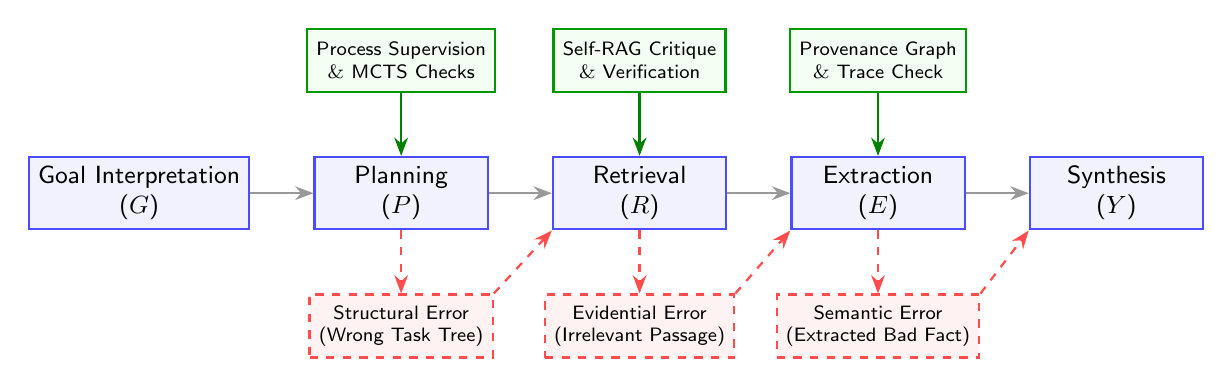
\begin{tikzpicture}[
    node distance=1.0cm and 0.8cm,
    stage/.style={rectangle, draw=blue!70, fill=blue!5, thick, minimum width=2.2cm, minimum height=0.9cm, align=center, font=\small\sffamily},
    error/.style={rectangle, draw=red!70, fill=red!5, dashed, thick, minimum width=2.0cm, minimum height=0.8cm, align=center, font=\scriptsize\sffamily},
    barrier/.style={rectangle, draw=green!60!black, fill=green!5, thick, minimum width=2.0cm, minimum height=0.8cm, align=center, font=\scriptsize\sffamily},
    arrow/.style={-Stealth, thick, color=gray!80},
    errorarrow/.style={-Stealth, thick, color=red!70, dashed}
]
    % Main Workflow Nodes
    \node (G) [stage] {Goal Interpretation\\($G$)};
    \node (P) [stage, right=of G] {Planning\\($P$)};
    \node (R) [stage, right=of P] {Retrieval\\($R$)};
    \node (E) [stage, right=of R] {Extraction\\($E$)};
    \node (Y) [stage, right=of E] {Synthesis\\($Y$)};

    % Arrows between main stages
    \draw [arrow] (G) -- (P);
    \draw [arrow] (P) -- (R);
    \draw [arrow] (R) -- (E);
    \draw [arrow] (E) -- (Y);

    % Propagation Mechanisms
    \node (E_struct) [error, below=0.8cm of P] {Structural Error\\(Wrong Task Tree)};
    \node (E_evid) [error, below=0.8cm of R] {Evidential Error\\(Irrelevant Passage)};
    \node (E_sem) [error, below=0.8cm of E] {Semantic Error\\(Extracted Bad Fact)};

    % Downward error creation arrows
    \draw [errorarrow] (P.south) -- (E_struct.north);
    \draw [errorarrow] (R.south) -- (E_evid.north);
    \draw [errorarrow] (E.south) -- (E_sem.north);

    % Forward error propagation arrows (diagonal from top-right corner to bottom-left of target stage)
    \draw [errorarrow] (E_struct.north east) -- (R.south west);
    \draw [errorarrow] (E_evid.north east) -- (E.south west);
    \draw [errorarrow] (E_sem.north east) -- (Y.south west);

    % Containment Barriers
    \node (B_proc) [barrier, above=0.8cm of P] {Process Supervision\\$\&$ MCTS Checks};
    \node (B_self) [barrier, above=0.8cm of R] {Self-RAG Critique\\$\&$ Verification};
    \node (B_prov) [barrier, above=0.8cm of E] {Provenance Graph\\$\&$ Trace Check};

    \draw [arrow, color=green!50!black] (B_proc.south) -- (P.north);
    \draw [arrow, color=green!50!black] (B_self.south) -- (R.north);
    \draw [arrow, color=green!50!black] (B_prov.south) -- (E.north);

\end{tikzpicture}
\caption{Taxonomy of error propagation channels (structural, evidential, semantic) and architectural containment barriers within a multi-step research automation workflow.}
\label{fig:taxonomy_workflow}
\end{figure*}

The AgentErrorTaxonomy developed by Zhu et al. \cite{zhu2025} provides a useful complementary classification, organizing failures into memory, reflection, planning, action, and system-level categories. Importantly, their trajectory-level analysis explicitly frames early errors as potential causes of downstream failures rather than treating each failure as an isolated event.

\subsection{Amplification versus Containment}

Propagation does not necessarily imply amplification. An intermediate error may be detected and corrected before affecting later stages. Therefore, an agentic workflow should be analyzed as a system containing both error channels and error barriers.

Let $q_i$ represent the probability that an error entering stage $i$ is detected and corrected. The effective propagation probability can be approximated conceptually as:
\begin{equation}
    P(E_{i+1} \mid E_i) = P(E_{i+1} \mid E_i, \text{undetected})[1-q_i].
    \label{eq:effective-propagation-probability}
\end{equation}
Verification, retrieval, external execution, cross-agent disagreement, human review, and process supervision can increase $q_i$.

This distinction is central to reliability engineering. A highly capable agent can still be unsafe if it lacks effective barriers, whereas a less capable agent can sometimes achieve higher end-to-end reliability when its architecture contains strong verification and recovery mechanisms.

\section{Error Propagation in Research Automation}

\subsection{Literature Discovery}

A typical research automation pipeline may begin:
\begin{equation}
    Q \rightarrow P \rightarrow R \rightarrow F,
    \label{eq:literature-discovery-pipeline}
\end{equation}
where $Q$ is the research question, $P$ is a search plan, $R$ is retrieved literature, and $F$ is a filtered evidence set.

Errors at the query interpretation or search-planning stage can cause systematic retrieval bias. Because later agents often operate only on the retrieved subset, downstream synthesis cannot necessarily recover information that was never retrieved. This creates an asymmetry between generation errors and coverage errors. A generation error may be corrected by checking the source. A coverage error may remain invisible because the missing evidence is not represented in the agent's state.

OpenScholar's use of a large scientific-paper corpus and retrieval-based synthesis illustrates an architectural response: increasing the breadth and quality of evidence access can reduce dependence on parametric model knowledge \cite{asai2024openscholar}. Yet the broader RAG literature indicates that retrieval itself remains a source of failure and does not guarantee faithful generation \cite{gao2023,huang2025}.

\subsection{Evidence Extraction}

Evidence extraction is a particularly high-leverage stage because extracted claims can be reused many times. Suppose a research agent processes 50 papers and incorrectly extracts a key effect estimate from one influential paper. If that estimate is later used in comparison, synthesis, hypothesis formation, and writing, one local error may generate several apparently independent errors.

This resembles error multiplication in data pipelines: the risk associated with an intermediate representation depends not only on its correctness but also on its downstream reuse count.

A useful concept is therefore the propagation centrality of an intermediate artifact:
\begin{equation}
    PC(x) = \sum_{j \in D(x)} w_j,
    \label{eq:propagation-centrality}
\end{equation}
where $D(x)$ is the set of downstream decisions dependent on artifact $x$, and $w_j$ represents the importance of each decision. High-centrality artifacts should receive stronger verification than low-impact intermediate outputs.

\subsection{Synthesis and Interpretation}

Research synthesis requires integrating heterogeneous findings rather than simply concatenating text. An agent may incorrectly infer that two studies are directly comparable when they use different populations, outcomes, or methodological assumptions. This produces a relational error: the individual facts may be correct, while the relationship inferred between them is false.

This distinction is important because conventional factuality evaluation often checks whether individual statements correspond to sources. Scientific synthesis additionally requires evaluating whether the inference connecting multiple sources is warranted.

Consequently, a citation-backed statement is not automatically a valid scientific conclusion. A reliable research agent must establish at least three relationships:
\begin{enumerate}
    \item the source exists;
    \item the source supports the cited factual statement; and
    \item the inference drawn from that statement is justified by the evidence.
\end{enumerate}

Self-RAG's critique mechanisms address the second problem more directly than the third, illustrating the need for research-specific reasoning verification beyond generic factuality checking \cite{asai2024selfrag}.

\subsection{Hypothesis Generation and Experimental Planning}

An error becomes potentially more consequential when a workflow transitions from information synthesis to action. A mistaken literature interpretation can lead an agent to formulate an invalid hypothesis, select inappropriate variables, or propose an experiment that does not test the intended proposition.

The risk therefore increases with semantic distance from the original evidence. Each transformation---from paper to extracted claim, claim to synthesis, synthesis to hypothesis, hypothesis to experimental design---creates another opportunity for distortion.

Agentic scientific-discovery surveys emphasize that autonomous research increasingly spans literature review, hypothesis generation, experiment design, analysis, and domain-specific discovery, but also identify reliability and validation as persistent barriers \cite{gridach2025}.

\section{Current Approaches and Developments}

Table~\ref{tab:lit_comparison} presents a comprehensive systematic comparison of primary agentic architectures, detailing their underlying error-mitigation mechanisms, supervision levels, key strengths, and open limitations.

\begin{table*}[htbp]
\caption{Comparative Analysis of Representative Reliability Mechanisms in Multi-Step Agentic AI Workflows}
\label{tab:lit_comparison}
\small
\centering
\begin{tabular}{p{2.2cm}p{2.8cm}p{1.8cm}p{3.2cm}p{3.2cm}}
\toprule
\textbf{Framework / Work} & \textbf{Core Mechanism} & \textbf{Supervision Level} & \textbf{Primary Strengths} & \textbf{Key Limitations} \\
\midrule
\textbf{ReAct} \cite{yao2023react} & Interleaved reasoning & Action-level & Interruption of faulty reasoning via real environment feedback & Susceptible to evidence misinterpretation and goal drifting \\
\addlinespace
\textbf{Self-RAG} \cite{asai2024selfrag} & Reflection tokens for adaptive retrieval & Step-level self-critique & Dynamic retrieval control; reduces hallucination in generation & Shares generator priors; vulnerable to correlated critique error \\
\addlinespace
\textbf{Reflexion} \cite{shinn2023} & Verbal reinforcement learning & Trajectory-level reflection & Non-gradient policy optimization; adaptive trial-and-error & May hallucinate rationales; high context window accumulation \\
\addlinespace
\textbf{Tree / Graph of Thoughts} \cite{yao2023tot,besta2024} & Multi-path exploration with lookahead search & State-level evaluation & Recovers from early branch errors via backtracking and merging & High computational latency; evaluation metrics can introduce bias \\
\addlinespace
\textbf{Process Supervision (PRM)} \cite{lightman2024,cobbe2021} & Step-by-step reward models & Step-level numerical reward & Pinpoints localized reasoning failures; improves complex problem solving & Annotations are expensive; limited generalization across non-math domains \\
\addlinespace
\textbf{AgentPro} \cite{deng2025} & Automated process supervision via MCTS & Step-level automated feedback & Prevents error cascade in multi-step agent reasoning chains & Dependent on quality of search heuristics and reward modeling \\
\addlinespace
\textbf{AgentDebug} \cite{zhu2025} & Causal error diagnosis taxonomy & Trajectory root-cause & Isolates origin of cascading failures across memory and planning & Post-hoc offline analysis; limited real-time runtime interventions \\
\addlinespace
\textbf{OpenScholar} \cite{asai2024openscholar,asai2026} & Citation-grounded scientific synthesis & Document-level provenance & Fact-checked citations; large datastore evidence synthesis & Focuses on literature review; does not handle complex experiment code execution \\
\bottomrule
\end{tabular}
\end{table*}

\subsection{Reasoning--Acting Architectures}

ReAct provides a foundational mitigation strategy by interleaving reasoning with external actions. Instead of generating a long reasoning chain without environmental feedback, the agent periodically acts, observes the result, and updates its plan \cite{yao2023react}.

For research automation, this suggests a closed-loop architecture:
\begin{equation}
    \text{Plan} \rightarrow \text{Retrieve} \rightarrow \text{Observe} \rightarrow \text{Verify} \rightarrow \text{Revise}.
    \label{eq:closed-loop-architecture}
\end{equation}
The advantage is that external evidence can interrupt a faulty internal trajectory. The limitation is that the agent may still misinterpret evidence or rationalize an incorrect plan.

\subsection{Self-Reflection and Verbal Feedback}

Reflexion introduced a mechanism in which agents use linguistic feedback to create reflective memories that influence subsequent attempts \cite{shinn2023}. This approach demonstrates that post-failure feedback can improve sequential decision-making without conventional gradient-based retraining.

For research workflows, reflection can be used after literature searches, evidence extraction, or synthesis. However, self-reflection is not equivalent to independent verification: the same model that generated the error may also generate the critique. This creates a risk of correlated evaluator error.

\subsection{Retrieval and Citation Grounding}

RAG and Self-RAG provide mechanisms for grounding generation in external evidence. Self-RAG is particularly relevant because it allows adaptive retrieval and self-critique rather than requiring indiscriminate retrieval for every generation step \cite{asai2024selfrag}.

For research automation, evidence-grounding systems should ideally retain a provenance graph:
\begin{equation}
    \text{Claim} \rightarrow \text{Evidence passage} \rightarrow \text{Paper} \rightarrow \text{Metadata}.
    \label{eq:provenance-graph}
\end{equation}
Such a structure allows downstream claims to be traced to their origins and makes error localization possible.

\subsection{Process Supervision and Verification}

Process supervision directly addresses a central weakness of outcome-only evaluation. Lightman et al. \cite{lightman2024} found that process supervision, which provides feedback on intermediate reasoning steps, outperformed outcome supervision in their evaluation of mathematical reasoning, while releasing PRM800K for step-level supervision research.

The general principle is highly relevant to agentic research:
\begin{equation}
    \text{Final correctness} \neq \text{intermediate correctness}.
    \label{eq:final-versus-intermediate-correctness}
\end{equation}
An agent can produce a correct final answer through a flawed path, or an incorrect answer because of a single flawed intermediate step. These cases have different implications for reliability and future reuse.

Verifier-based methods similarly demonstrate that an independent model can evaluate candidate solutions and select among them \cite{cobbe2021}. However, research workflows require verifiers capable of evaluating evidence relevance, citation entailment, methodological comparability, statistical validity, and inference quality---not merely final-answer correctness.

\subsection{Search over Alternative Reasoning Paths}

Tree-of-Thoughts enables agents to explore multiple candidate reasoning trajectories and backtrack when a path appears unpromising \cite{yao2023tot}.

Graph-of-Thoughts extends this approach by representing reasoning units and their dependencies as graphs, allowing aggregation and feedback across reasoning paths \cite{besta2024}.

For research automation, branching can reduce the chance that a single early decision irreversibly determines the entire workflow. However, branching does not automatically produce independent evidence. If multiple paths originate from the same incorrect assumption, apparent consensus can be misleading.

\subsection{Automated Process Supervision and Debugging}

AgentPro operationalizes process supervision using Monte Carlo Tree Search, step-level annotations, and a process reward model to prevent agents from continuing along erroneous reasoning trajectories \cite{deng2025}.

AgentDebug takes a complementary trajectory-level approach. Its AgentErrorTaxonomy categorizes failures across memory, reflection, planning, action, and system operations, while AgentErrorBench provides annotated failure trajectories. The proposed debugging framework seeks to identify root causes rather than merely reacting to final task failure \cite{zhu2025}.

These developments indicate a shift from performance optimization toward failure diagnosis, which is essential for mature research automation.

\section{A Reliability Framework for Agentic Research Workflows}

A robust research agent should be conceptualized as a sequence of states connected by evidence and decisions:
\begin{equation}
    G \rightarrow P \rightarrow S \rightarrow R \rightarrow E \rightarrow Y \rightarrow V,
    \label{eq:agentic-research-state-sequence}
\end{equation}
where $G$ is goal interpretation, $P$ is planning, $S$ is search, $R$ is retrieval, $E$ is evidence extraction, $Y$ is synthesis or inference, and $V$ is verification. Each node can have local errors, while edges represent propagation channels.

\subsection{Step Reliability}

For each stage $i$, define step reliability $r_i$ as:
\begin{equation}
    r_i = P(C_i = 1).
    \label{eq:step-reliability}
\end{equation}
Traditional evaluation estimates $r_i$ independently. Agentic reliability requires additionally estimating conditional step reliability $r_{i \mid j}$:
\begin{equation}
    r_{i \mid j} = P(C_i = 1 \mid C_j = 0),
    \label{eq:conditional-step-reliability}
\end{equation}
which measures how much a prior failure changes downstream correctness.

\subsection{Propagation Coefficient}

A practical metric can be defined as:
\begin{equation}
    \gamma_{j \rightarrow i} = P(E_i \mid E_j) - P(E_i \mid \neg E_j).
    \label{eq:propagation-coefficient}
\end{equation}
A positive $\gamma$ indicates that an earlier error increases downstream error probability.

For example, if downstream extraction errors occur in 20\% of trajectories when search is correct but in 60\% when search contains a specific error, the estimated propagation coefficient is 0.40.

\subsection{Error Severity}

Not all errors are equally damaging. A minor formatting error and an incorrect causal conclusion should not receive the same weight. Define severity $s_i$ as a function of scientific consequence, downstream reuse, reversibility, and detectability:
\begin{equation}
    s_i = f(I_i, D_i, R_i, U_i),
    \label{eq:error-severity}
\end{equation}
where $I_i$ is impact, $D_i$ is downstream dependency, $R_i$ is reversibility, and $U_i$ is difficulty of detection.

A research agent should prioritize verification at high-severity nodes rather than applying uniform verification to every generated token.

\subsection{Recovery Probability}

A critical but under-measured property is the ability to recover:
\begin{equation}
    \rho_i = P(\text{successful recovery} \mid E_i).
    \label{eq:recovery-probability}
\end{equation}
Two systems with identical failure rates can have radically different reliability if one can detect and repair failures before they contaminate downstream states.

Accordingly, an evaluation suite for research agents should report at least: step accuracy, end-to-end success, error-detection rate, root-cause localization accuracy, propagation coefficient, recovery rate, time/cost per successful task, citation correctness, evidence coverage, and calibration/abstention quality.

\section{Research Challenges and Limitations}

\subsection{Correlated Errors}

The independence assumption is often unrealistic. Multiple agents may share the same base model, retrieval corpus, prompt templates, or hidden biases. Consequently, majority voting among agents does not necessarily produce independent evidence.

This is particularly important for multi-agent research systems. Three agents agreeing on an unsupported claim may represent one shared model prior rather than three independent confirmations.

\subsection{Evaluator Reliability}

Self-critique and LLM-as-judge methods introduce another agent whose errors can propagate into the evaluation process. If the evaluator shares the same blind spot as the generator, the system can incorrectly certify a flawed result.

Process supervision therefore requires carefully designed evaluators, preferably incorporating heterogeneous evidence sources, deterministic checks, external databases, executable tests, or human review where appropriate.

\subsection{Dynamic Research Environments}

Research agents frequently operate over changing online information. Web search results, APIs, databases, and document versions can change over time. BrowseComp illustrates the challenge of evaluating browsing agents that must persistently navigate large and changing information spaces \cite{wei2025}.

This creates a reproducibility problem: the same agent and query may not produce the same evidence set at different times.

\subsection{Citation Correctness versus Scientific Validity}

Citation evaluation is necessary but insufficient. A citation may correctly point to a real paper while failing to support the precise proposition made by the agent. More subtly, multiple individually supported propositions can be combined into an unsupported causal or theoretical conclusion.

Scientific agents therefore require argument-level verification, not only citation-level verification.

\subsection{Long-Horizon Degradation}

AgentBench and WebArena demonstrate that performance can deteriorate substantially when tasks require extended interaction and decision-making \cite{liu2024,zhou2024}. Long-horizon research workflows may contain dozens or hundreds of intermediate operations, magnifying the probability that at least one important state becomes corrupted.

\subsection{Benchmark Limitations}

Existing benchmarks differ substantially in environment, task length, evaluation criteria, and degree of human involvement. Agent evaluation research increasingly recognizes the need for realistic and fine-grained benchmarks, but standardized metrics for propagation, recovery, and scientific validity remain underdeveloped \cite{yehudai2026}.

\section{Research Gaps and Future Directions}

\subsection{From Final-Answer Evaluation to Trajectory Evaluation}

The most important research gap is methodological. Current evaluations frequently ask whether an agent ultimately succeeded. A scientifically useful evaluation should instead ask: Where did the trajectory first become unreliable, how did that error propagate, and could the system have recovered?

Trajectory-level evaluation should preserve every action, observation, retrieved source, intermediate claim, tool result, and state transition.

\subsection{Provenance-Aware Agent Memory}

Research agents should store not only information but its provenance. A memory item should ideally encode:
\begin{equation}
    M = (c, e, s, t, q),
    \label{eq:provenance-aware-memory}
\end{equation}
where $c$ is the claim, $e$ is supporting evidence, $s$ is source identity, $t$ is acquisition time, and $q$ is confidence or verification status.

This would allow an agent to distinguish directly verified facts, model-generated hypotheses, uncertain interpretations, externally validated calculations, and unresolved claims. Such typed memory could substantially reduce the tendency for speculative outputs to become permanent facts in later workflow stages.

\subsection{Causal Error Attribution}

AgentDebug demonstrates the value of root-cause analysis \cite{zhu2025}. Future systems should formalize this using causal graphs over trajectories. A trajectory could be represented as:
\begin{equation}
    X_1 \rightarrow X_2 \rightarrow \cdots \rightarrow X_N,
    \label{eq:causal-trajectory}
\end{equation}
with additional cross-links for shared evidence and memory. Interventions on earlier states could then estimate whether changing a particular state would have prevented final failure. This would move agent debugging from correlation toward causal diagnosis.

\subsection{Adaptive Verification}

Uniform verification is expensive. A more scalable approach is risk-adaptive verification:
\begin{equation}
    V_i = f(p_i, s_i, d_i, u_i),
    \label{eq:risk-adaptive-verification}
\end{equation}
where verification intensity $V_i$ depends on estimated correctness $p_i$, severity $s_i$, downstream dependency $d_i$, and uncertainty $u_i$.

High-impact claims---for example, the numerical result driving a meta-analysis or the premise underlying an experimental recommendation---should receive stronger checks than low-impact formatting operations.

\subsection{Independent Evidence Triangulation}

Future research agents should distinguish between model diversity and evidence diversity. Multiple agents using the same source corpus are not truly independent. Stronger verification could require agreement across heterogeneous channels including primary research papers, structured databases, executable calculations, statistical tests, domain-specific knowledge bases, independent retrieval systems, and human experts.

\subsection{Recovery-Aware Architecture}

Instead of assuming that every workflow should proceed linearly, agents should maintain explicit recovery states:
\begin{equation}
    \text{Execute} \rightarrow \text{Detect} \rightarrow \text{Localize} \rightarrow \text{Rollback} \rightarrow \text{Retry}.
    \label{eq:recovery-aware-architecture}
\end{equation}
Rollback is especially important. If a faulty evidence extraction contaminates five subsequent steps, simply correcting the final answer may leave corrupted intermediate memory intact. Reliable systems should be able to invalidate downstream states that depend on the corrected artifact.

\subsection{Research-Specific Benchmarks}

A major future contribution would be a benchmark explicitly designed around scientific error propagation. A suitable benchmark should contain long-horizon tasks with known ground-truth provenance graphs and controlled perturbations (e.g., injected incorrect metadata, misleading abstracts, citation substitutions, numerical extraction errors, or tool failures).

The benchmark could then measure whether an agent detects, propagates, corrects, or amplifies each perturbation. Such controlled experiments would make it possible to estimate propagation coefficients rather than relying solely on final task success.

\subsection{Human Oversight as a Targeted Reliability Mechanism}

Human-in-the-loop systems should concentrate intervention at high-risk boundaries such as transitions from evidence to causal inference, experimental recommendations, decisions involving irreversible actions, contradictory evidence, low-confidence synthesis, or claims with unusually high downstream dependency.

This produces a selective oversight architecture in which automation handles routine transformations while human expertise is allocated to uncertainty and consequence.

\section{Conclusion}

Multi-step agentic AI offers a compelling pathway toward research automation, but its reliability cannot be inferred from the accuracy of the underlying language model or from isolated tool-use benchmarks. Research workflows are dependency networks in which intermediate outputs become inputs to subsequent decisions. Consequently, a local error can become a system-level failure through semantic, structural, evidential, or operational propagation.

The literature already provides several mechanisms for reducing this risk. ReAct introduces closed-loop reasoning and acting; RAG and Self-RAG improve access to external evidence and enable retrieval-aware critique; Reflexion supports learning from feedback; Tree-of-Thoughts and Graph-of-Thoughts enable alternative reasoning paths; process supervision and verifier models evaluate intermediate states; and recent trajectory-level systems such as AgentPro and AgentDebug explicitly target intermediate failures and cascading errors \cite{yao2023react,asai2024selfrag,shinn2023,lightman2024,deng2025,zhu2025}.

Nevertheless, important gaps remain. Current evaluation is still disproportionately focused on final outcomes rather than the causal structure of trajectories. Research automation additionally requires evidence provenance, source coverage, methodological validity, inference checking, uncertainty estimation, and recovery from intermediate failures. These requirements are more stringent than conventional chatbot factuality.

The central implication is therefore architectural: reliable agentic research automation should be designed as a fault-aware workflow rather than as a sequence of increasingly capable language-model calls. Future systems should maintain provenance-rich state, quantify step-level reliability, detect high-impact anomalies, verify critical intermediate claims, attribute failures to their roots, invalidate contaminated downstream states, and recover through controlled replanning.

The ultimate research objective should not be to construct agents that never make mistakes---a practically unrealistic goal---but agents in which mistakes are observable, localized, bounded, recoverable, and prevented from silently becoming scientific conclusions. Such a shift from capability-centric development to reliability-centric engineering is likely to be essential if autonomous research systems are to progress from useful assistants toward trustworthy components of the scientific process.

\bibliographystyle{ACM-Reference-Format}
\bibliography{references}

\end{document}

